\documentclass[sigconf, nonacm]{acmart}
\usepackage{balance}
\usepackage{booktabs}
\usepackage{multirow}
\usepackage{array}

\newenvironment{conditions}
  {\par\vspace{\abovedisplayskip}\noindent\begin{tabular}{>{$}l<{$} @{${}={}$} l}}
  {\end{tabular}\par\vspace{\belowdisplayskip}}

\begin{document}
\title{Home Loan Default Prediction with Machine Learning}

%%
%% The "author" command and its associated commands are used to define the authors and their affiliations.
\author{Sakib Sadman Shajib}
\affiliation{%
	\institution{North South University}
	\department{Department of Electrical and Computer Engineering}
}
\email{sakib.shajib173@northsouth.edu}

\author{Ilmiat Farhana}
\affiliation{%
	\institution{North South University}
	\department{Department of Electrical and Computer Engineering}
}
\email{ilmia.farhana@northsouth.edu}

\author{Tahmid Hasan Nafi}
\affiliation{%
	\institution{North South University}
	\department{Department of Electrical and Computer Engineering}
}
\email{tahmid.nafi@northsouth.edu}

\author{Iftekhar Alam Pial}
\affiliation{%
	\institution{North South University}
	\department{Department of Electrical and Computer Engineering}
}
\email{iftekhar.pial@northsouth.edu}

\begin{abstract}

Data is increasingly being generated worldwide. And this data, when processed, can speak a lot about us. Correspondingly, financial data can speak a lot about a person's financial credibility. Credit scores are what serve that very purpose. A person with an incomplete or non-existent credit history has low credibility due to lack of data. And therefore have less probability of obtaining approval for home loans. But if we incorporate alternate data sources to their incomplete or non-existent credit history, we can acquire an eagle-eye view about their financial situation. Therefore, we used machine learning to predict their credibility using their credit history, loan application and alternate data sources. In order to establish our concept, we have used a data-set provided by Home Credit International for a Kaggle competition. In spite of the fact that, this concept is nothing new, we have improved the data processing pipeline by creating more relevant features via feature engineering. Additionally we have trained different types of machine learning models such as, linear, ensembles, gradient boosting, deep learning for tabular data and neural networks. We have also used model tuning tools to find the best parameters with the best score. Our best performing model has an AUC-ROC score of 80.12\%.

\end{abstract}

\maketitle

\section{Introduction}

The goal of our research is to help lenders take data-driven decisions for applicants with incomplete credit history. Incomplete credit history refers to the fact that the applicants do not have a fully detailed history about their previous loans or have inaccuracies in their credit or purchase management record. We are working with a data-set provided by Home Credit International, a company that provides financial facilities for purchasing real-estate, for a Kaggle(an online community of data scientists and machine learning practitioners) competition to assess risk, based on incomplete or unavailable credit history paired with alternative data sources. The data-set provides us with a few alternate data sources such as credit card's usage information, previous application and history of payment, its usage and status, and also data from the credit bureau.

\paragraph{Advantages of Home Loan}
Usually a bank will provide loan who has better credit history but often it is important to give loan a person who has an incomplete or no credit history. The factors behind this are stated below:
\begin{itemize}
	\item If a person does not use credit from the system, he will not be able to create a credit history. So, if a customer has no credit history, he may be in the process of establishing credit.
	\item The home loan makes it easier for a person with an average middle-class salary, to buy a home of their own.
	\item In the financial industry, people will have better knowledge.
	\item This is another significant benefit of availing a home loan. If you have mortgaged property against a loan, you could claim a tax deduction on the principal as well as the interest part of the repayment.
	\item It decreases the percentage of unemployment.
\end{itemize}

\paragraph{Disadvantages of Home Loan}
There may also be some drawbacks of taking a home loan. These drawbacks mostly affect the client. The details are shown below:
\begin{itemize}
	\item This is a Significant Commitment:
	      When a lender approves customer's home loan application, the customer is making a significant long-term commitment. A home loan is typically for a span of years. This implies that he will be in debt for a major portion of his life. He must be prepared to manage his spending and focus on repayment once the loan is in place.
	\item A Home Loan May Involve Risks:
	      The average home loan lasts between 10 and 30 years, which is quite a long period. Several unforeseeable events may occur during this time. Some of these circumstances could make repaying the loan difficult.
	\item Loss of investment opportunity:
	      One of the most underappreciated drawbacks of a home loan is loss of investment opportunity. When someone applies for a loan, regardless of the magnitude of the amount loaned is, or how long or short the repayment period is, he forfeits the chance to invest the same money in an investing instrument that may provide him with excellent returns.
\end{itemize}

In our proposed Loan Prediction System, we have checked the eligibility of particular customers who have the credibility to apply for loans. This system checks parameters like the customer’s age, marital status, income, expenditure, etc. Taking these factors into account, a required model is built. This model is then applied on the test data-set for achieving the required output. Based on these factors we can approve home loans for customers. Our project aims to use domain knowledge feature engineering, in combination
with standard classification algorithms to obtain a predictive model, and compare their performances.

\section{Relevant Works}
In this section, some of the works that were previously done in this area are discussed.

Ziyue Qiu et al. \cite{9107890} has used LightGBM, Logistic Regression, Random Forest models in their paper and concluded that for credit risk scoring models, no matter what the feature construction method is, generally the model performance is LightGBM \textgreater  Logistic Regression \textgreater  Random Forest. Their best model achieved 78\% of the AUC score on Kaggle Home Credit Default Risk data-set. They discarded features that contain over 70\% percent of null values and implied two methods of missing data, i.e. Imputation: mean imputation/medium imputation, and Random Forest imputation. 

In another study, Yiyun Liang et al. \cite{Liang2019LoanlinessPL} had similar findings. They used sampling methods on the data-set to show that Downsampling helped achieve the best performance. We acknowledge the fact that the data-set they used, was very challenging and heavily imbalanced. They experimented with a number of models, i.e. Random forest, LGBM, Logistic Regression, Naive bayes, MLP and also performed clustering via K-means. Their best overall performance was with a value of k=4 and for each one of the four clusters. The LightGBM model performs the best(71.57\%) out of all the  machine learning models that they have worked with.


Xue Chen et al. \cite{10.1145/3366194.3366333} introduced the latest deep learning framework DeepGBM for a better performance on this data-set. It compares DeepGBM with PNN, Random forest, LGBM  and shows that DeepGBM gives better result(0.756) compared to traditional singular classifiers. It combines the best of both neural networks and GBDT. DeepGBM is a GB system based on deep learning. Recently proposed by Guolin Ke, DeepGBM\cite{deepgbm} has a good trade-off between sparse classification features and dense numerical features. 

The most significant drawback of this paper was that they used only two of the seven csv files application\_train.csv, and application\_test.csv files in their experiments. This means that they worked with only 104 features, whereas in our paper we included all the files and came up with way more features.


The primary goal of Ravid et al. \cite{shwartzziv2021tabular}   was to determine whether any of the given deep models should be recommended for tabular data-set issues. It showed that each model performs best on the data-sets used in its respective papers but considerably worse on alternative data-sets in most situations. The research demonstrates that XGBoost consistently outperforms deep models on these data-sets. Also, the hyper-parameter search procedure for XGBoost was considerably faster. On the other hand, they compared the performance of a deep model ensemble coupled with XGBoost and figured that this ensemble produces the best results. The ensemble of deep models and XGBoost outperforms the other models in most cases. However, the paper should have experimented with more models to compare with its best result. Which, in turn, would ensure a clearer idea on which classifier combination provides the better performance.



While in most of the papers, single classifiers are used to solve the credit evaluation problem,  Zhenlong Liu et al. \cite{liu_zhang_2021} claims that their proposed model which is the combination of GBDT2NN (Gradient Boosting Decision Tree to Neural Network) and FM (Factorization Machine) gives better performance than single classifiers, i.e. GBDT2NN, LGBM, Logistic Regression. They also proposed an interesting method named SMOTE((Synthetic Minority Over-sampling Technique) to solve the imbalance between the categories in the classification. And while this method improves the balance of the data-set, it also increases the difficulty of the classification algorithm.

Another comparison between two machine learning models MLP(Multi-Layer Perceptron) and CNN(Convolutional Neural Networks) were made by  Salomey et al. \cite{Osei_2021} for credit risk . In their experiments, CNN came out to be the better model for accuracy and other performance metrics used,such as, back-testing,stress testing. We can also see that MLP method could do better with parameter tuning.


In our paper we implemented  binary classifiers using linear models, Gradient boosting methods, combinations of classifier models, sampling methods and Neural embedding methods, which we then compared to make a claim of which method or model gives the best performance. Our research was to create more features from existing data. We tried different model comparisons and acquired better scores .

\section{Methodology}
\subsection{Data Source}
Home credit is an international consumer financial service provider, founded in 1997 in the Czech Republic with its headquarters in the Netherlands and operations in ten other countries. It is a financial organization that provides loans to those who have a poor credit history.
The data\cite{data-set} is a historical data-set based on actual clients and loans provided for Home Credit Default Risk for Kaggle competition, collected over different time frames and sources. Only credit default data from the United States was used in this investigation. Kaggle is a prominent data science (DS) platform owned by Google. DS competitions can be hosted or participated in, by data scientists, researchers, and developers. Users can enter competitions and submit answers to data-set-specific challenges. Home credit launched this challenge in Kaggle 3 years ago, for researchers to help them unlock the full potential of their data.
We chose this data-set for our research vastly because of the huge collection of data it provides.

We do, however, have other useful information, such as their credit bureau balance and credit card history. We have 122 columns of data that contain fields such as annual income, number of children, gender, number of days of employment at their workplace, age in days, etc.

% Start

\subsection{Pre-Processing and Feature Engineering Pipeline} \label{subsec:feat_eng}

\subsubsection{Version 1} \label{data:v1}
Some basic pre-processing techniques were enforced to prepare the data for our Machine Learning Models.

\paragraph{Application}

The fundamental step was to remove the untrue/ impossible data. For example, the data in which, an application was submitted 365243 days before they started a job. This means that the person will need to live for more than 1018 years. Another example would be that of a person with an yearly income of more than 20 Million USD applying for the loan with an incomplete credit history.

Entries with incomplete important features, such as Gender or the number of days before which the client changed their phone number prior to submitting application, were removed.

Ages were classified into groups and a numerical label was assigned to each group in order to portray a better representation of age.

There are a few normalized features named EXT\_SOURCE\_X. These features are either credit scores or equivalents from external sources. Some features were created by carrying out statistical operations among them. These operations include the product, the weighted average, the minimum or maximum, the mean, the median (including blank data) and the variance.

Some meaningful ratios between features, such as, amount of loan vs existing credit, amount of loan vs collateral value, existing credit vs annual income, and amount of loan vs annual income, were established.

Another way of creating new features is by carrying out statistical operations such as the mean, the median, the standard deviation and the sum, using features which can be used as groups, i.e., ORGANIZATION\_TYPE, NAME\_EDUCATION\_TYPE, OCCUPATION\_TYPE, AGE\_RANGE and CODE\_GENDER.

Features having very low correlation with the label "TARGET" were eliminated.

Label Encoding\cite{pandas.factorize} was used to encode the categorical features.

\paragraph{Bureau}

New features were created, i.e., loan duration, change of End date, debt percentage, difference between current loan and amount of loan applied. Some ratios between connected data for example, bureau reported loan vs loan amount, were also created.

One-Hot Encoding\cite{sklearn.preprocessing.onehotencoder} was used for encoding the categorical features.

A summation of the statuses of each applicant were taken into account and a new feature named "STATUS\_12345" was created. This feature helps flag months in which the payment made, was pending or delayed.

The data used were classified into groups, based on the magnitude of the monthly balance. This was done to detect the number of months left for the payment of previous loans. This information was then merged with the bureau data. General loans were grouped in "bureau" data and new features were created by carrying out statistical operations. Active and Closed loans were taken into account as well. More features were created by aggregating the types of loan and creating another time based aggregation.

Another important feature was to find out, the the last loan's maximum overdue. And finally more ratio based features were created and merged with the application data

\paragraph{Previous Application}

The categorical data was encoded using Label Encoding\cite{pandas.factorize}. And features were created based on ratios and difference. Another feature was also created, to find the simplified interest ratio on the last applications.

All the active loans, that were approved but not completed, were listed. The actual amount that was paid as well as the impending amount, was calculated. Then this data was merged with the application data.

A recurring pattern of the number 365243 was found. This was because this number is what the data-set represents as infinity or garbage info. Every instance of the number was then removed.

The date was aggregated and new features were created, by carrying out statistical operation. The same was done for loans which are active and were refused, consumer and cash loans, loans with late payments, and for loans in the last 2 years. The resulting data was then merged with application data.

\paragraph{Final Processing}

The label "TARGET" was removed from the data along with all positive and negative infinities. 460 features remained in the data-set afterwards.

\subsubsection{Version 1.1}\label{data:v1.1}

In \ref{data:v1}, More data was used from the data source.

\paragraph{POS and Cash}

The process began with flagging late payments, as well as, grouping and sorting the data, using the indexes. Percentage of loans that were paid off before the due date were listed. The number of the remaining was also listed.  
\emph{Each Month Installments} (EMI) that are remaining as well as the percentage of the EMI already paid, was also computed. These lists were then used to aggregate the data using the indexes.

The percentage of late payments in the 3 recent late payments, were found, along with the last month's credit card balance of each application. A new feature was then created, which calculated the mean of the balance for the last 3 months.

Finally some irrelevant features were eliminated. This data was also merged with our current pipeline.

\paragraph{Installments}

The payments were grouped against their loan application IDs and the difference between the monthly payments were computed. Entries were made, of the payments which were made before and after the due date. And the late payments were flagged. The percentage of late payments were computed. Late payments that have significant impending amounts were flagged. Flags were also set up based on how late the payments were, ranging from 7 days and 15 days thresholds. All this was then aggregated using the indexes.

The installments in the last 3 to 5 years were grouped. New features were created using these groups, and by carrying out statistical operations on them. The payment trends on the recent payments such as delay or advance, under or over payment, were also figured. Some features were created, relating to the previous loan's installments.

\paragraph{Credit Card}

Features that keep record of the amount of limit used, the current payment vs the minimum payment ration, if there are any late payments and the amount of delay, ratio of cash draw vs limit, were created. The last month's balance of each credit card of the applicant was recorded, and aggregated with the monthly balance of last 3 years.

\paragraph{Improvement from previous version}

The new pipeline has \emph{649 features} in total. And it has more related information about the applicants financial situation.

\subsection{Model}
Some Binary Classifier models were trained to find the probability of default-ability of an applicant using the data-set.

\subsubsection{Logistic Regression} \label{subsubsec:log_reg}
Initially a linear model was used, as our data shows good correlation. Many new features were extracted from the processed data. A Logistic Regression\cite{10.1001/jama.2016.7653} model was trained. Logistic Regression is a statistical model that uses logistic at it's base, shown in Equation \ref{eqn:log_func}, to create a Binary Classifier.

\begin{equation}
	f(x) = \frac{L}{1 + e^{-k(x-x_0)}}
	\label{eqn:log_func}
\end{equation}

\paragraph{Data Pipeline}
A Simple Imputer\cite{sklearn.impute.simpleimputer} model was used to impute the blank data and use a Min-Max Scaler model\cite{sklearn.preprocessing.minmaxscaler} to scale the data from 0 to 1.

\paragraph{Training}
The parameter used for the Logistic Regression model is C=0.0001, which is the inverse of the regularization strength. A lower C value means greater the regularization strength.

\paragraph{Scores}
We used both versions of our data processing pipeline and got these AUC-ROC scores in Table \ref{tab:log_reg}.

\subsubsection{Random Forest}

Random Forest\cite{sklearn.ensemble.randomforestclassifier} is an ensemble model of multiple Decision Trees. The model trains multiple trees and then through major voting outputs a prediction. A visual representation of how the model works is provided in Figure \ref{fig:ran_for}

\paragraph{Data Pipeline and Model Training}
Random Forest is a very popular classifier model for tabular data. So, we have trained a Random Forest Classifier model using our Processed Data (\ref{subsec:feat_eng}), using similar imputer and normalizer models to \ref{subsubsec:log_reg}.
\begin{figure}[t]
    \centering
    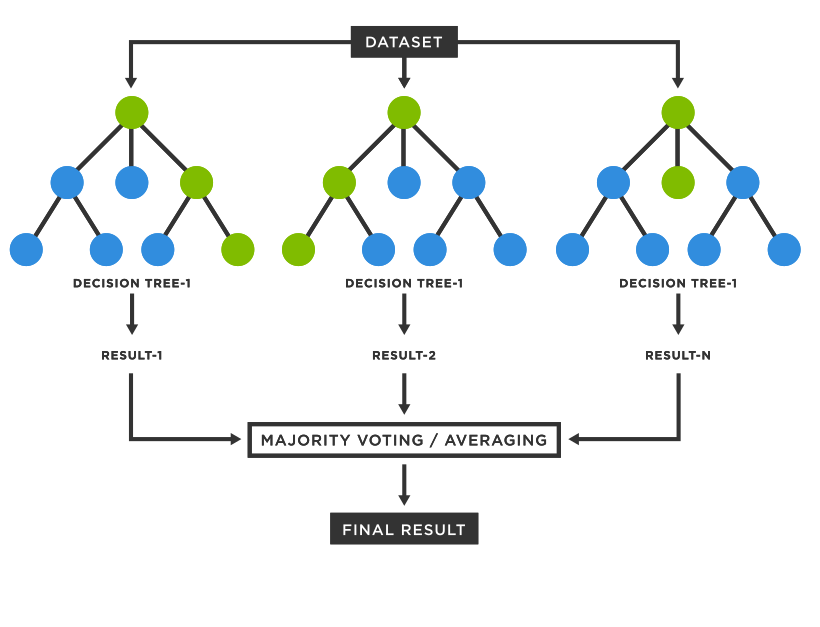
\includegraphics[width=0.45\textwidth]{random_forest/random-forest-diagram.png}
    \caption{Random Forest}
    \label{fig:ran_for}
\end{figure}

\paragraph{Scores}
The AUC-ROC scores with their corresponding parameters can be found in Table \ref{tab:ran_for}

\subsubsection{LightGBM} \label{subsubsec:lgb}

Light Gradient Boosting Machine\cite{Ke2017LightGBMAH} is a relatively new framework developed by Microsoft. It is a gradient boosting tree based learning algorithm.

A decision tree algorithm can predict class or value by inferring simple binary decision rules from data. A decision tree grows level-wise (depth-first) as shown in Figure \ref{fig:lgb_level}, the decision tree that we used, grows vertically, i.e. leaf-wise (best-first) as shown in Figure \ref{fig:lgb_leaf}. It uses the leaf with the max delta loss, i.e. the leaf that has the largest decrease in the cost function, in order to grow. When growing best-first, the trees can grow much faster compared to depth-first.

\begin{figure}[h]
	\centering
	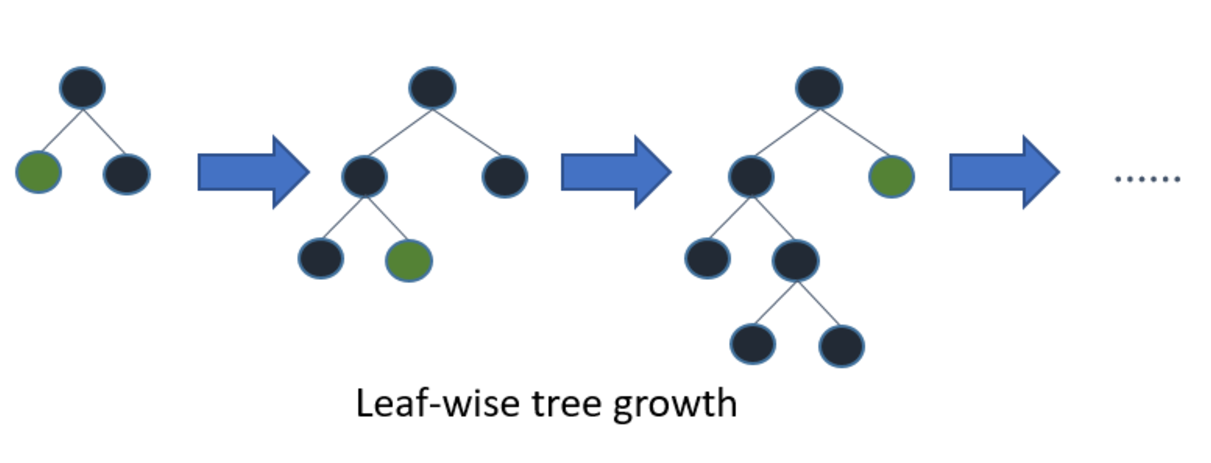
\includegraphics[width=0.45\textwidth]{lgb/1_AZsSoXb8lc5N6mnhqX5JCg.png}
	\caption{Leaf-wise tree growth}
	\label{fig:lgb_leaf}
\end{figure}

\begin{figure}[h]
	\centering
	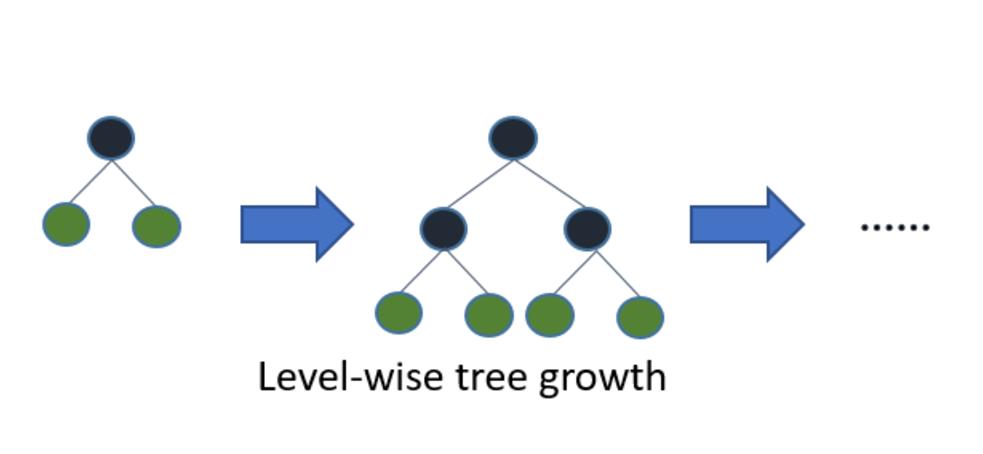
\includegraphics[width=0.45\textwidth]{lgb/1_whSa8rY4sgFQj1rEcWr8Ag.png}
	\caption{Level-wise tree growth}
	\label{fig:lgb_level}
\end{figure}

LightGBM does not use sorted-based decision tree, which searches the best split point on sorted feature values. Instead it uses a highly optimized version of histogram-based decision tree learning algorithm.

\paragraph{Boosting}
Experiments were carried out with \emph{Gradient-Based One-Side Sampling} (GOSS) as the boosting method, which is memory-efficient and makes training the model faster. GOSS works with the principal that features with larger gradients have more effect on the information gain, thus it randomly drops features with smaller gradients still retaining the accuracy.

\paragraph{Data Pipeline}
The model was trained using data from our Data Pipeline (\ref{subsec:feat_eng}). The data was imputed using a simple imputer model\cite{sklearn.impute.simpleimputer} to remove all the blank features using median of the feature-set. And for experiment, we scaled the data using a minmax scaler\cite{sklearn.preprocessing.minmaxscaler} model to convert the data range from 0 to 1, although this decreases the accuracy of the model.

\paragraph{Training}
The training data was divided into 5 Folds and each fold was trained and validated, using our evaluation metrics \emph{Area Under the curve of Receiver Operating Characteristic curve} (AUC-ROC). Then the best iteration was used to predict the test feature-set. \label{kfold}

The model \cite{parameters_tuning_lightgbm} was tuned using Grid Search Cross Validation\cite{sklearn.model_selection.gridsearchcv} was used to find the hyper-parameters\cite{parameters_lightgbm} for the best result.

\paragraph{Scores}
The parameters used and the corresponding AUC-ROC score are given in Table \ref{tab:lgb}.

\subsubsection{XGBoost} \label{subsubsec:xgb}

XGBoost\cite{Chen_2016} is a very popular gradient boosting decision tree\cite{friedman2001greedy} based learning algorithm. It is used for supervised learning problem, where use a tabular data with multiple features to predict a target label. XGBoost names implies Extreme Gradient Boosting.

XGBoost divides the optimization into two parts. The first is determining the direction of the step (Equation \ref{eqn:boost}) and then optimize the step length.\cite{xgboost_2021}

\begin{equation}
	\label{eqn:boost}
	f(x) = \sum_{m=0}^{M} f_m (x) = f_0 (x) + \sum_{m=1}{M} \theta_{m} \phi_{m} (x)
\end{equation}\cite{gbm_2021}
where:
\begin{conditions}
	f_0                   &   the initial guess                   \\
	\phi_m (x)            &   the base estimator at iteration $m$ \\
	\theta_m              &   the weight for the $m^{th}$ estimator \\
	\theta_{m} \phi_{m}   &   the step at iteration $m$           \\
			    
\end{conditions}

\paragraph{Data Pipeline}
Both versions of Data Processing Pipeline were used in \ref{subsec:feat_eng}. The data was imputed and normalized using a median based Imputer model and a range -1 to 1 MinMax Scaler model respectively.

\paragraph{Training Model}
Initially the model was trained by splitting the training data into 80:20 into train and validation data. But then it was came into view that the accuracy could be improved by training the model using folds. Thus 5 Folds were used to train the model with the previous parameters and saw marginal improvements.

Then the Grid Search Cross Validation\cite{sklearn.model_selection.gridsearchcv} was used to fine-tune\cite{xgboost_parameters_2021} the hyper-parameters to get the best results.

Finally, XGBoost's GPU supported\cite{xgboost_gpu_support_2021} histogram learning tree method\cite{xgboost_tree_methods_2021} was used. The training time was drastically reduced and got a better score.

\paragraph{Scores}
The parameters used and the corresponding AUC-ROC scores are given in table \ref{tab:xgb}

\subsubsection{TabNet} \label{subsubsec:tabnet}

TabNet\cite{arik2020tabnet} is a \emph{Deep Neural Network} (DNN) for tabular structured data developed by Google Cloud AI Team. The paper\cite{arik2020tabnet} mentions that Decision Tree Ensembles (LightGBM\cite{Ke2017LightGBMAH}, XGBoost\cite{Chen_2016}) and lack of equal performing Neural Network classifiers.

TabNet uses a Decision Tree like classifier (Figure \ref{fig:dt_like_class}) and decision manifold (Figure \ref{fig:dec_man}). It has an advanced feature selection which uses sequential attention to give feature weights in each decision steps.

\begin{figure}[h]
	\centering
	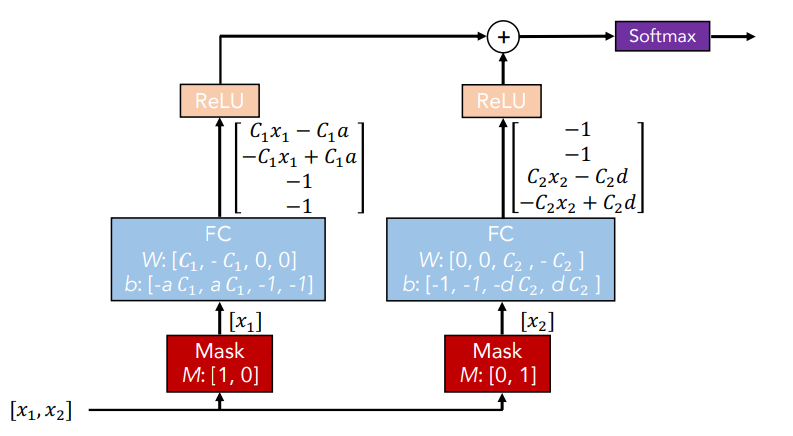
\includegraphics[width=0.45\textwidth]{tabnet/1908.07442-1.png}
	\caption{Illustration of DT-like classification using conventional DNN blocks}
	\label{fig:dt_like_class}
\end{figure}

\begin{figure}[h]
	\centering
	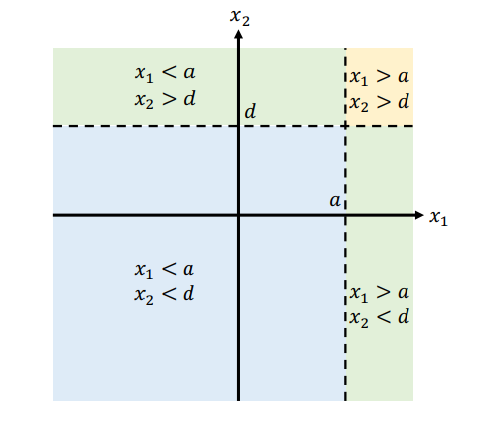
\includegraphics[width=0.45\textwidth]{tabnet/1908.07442-2.png}
	\caption{Decision Manifold}
	\label{fig:dec_man}
\end{figure}

\paragraph{Data Pipeline, Model Training \& Tuning}
The Data Pipeline and Model Training similar to XGBoost models' \ref{subsubsec:xgb}'s Data Pipeline and Model Training respectively. We also used Grid Search CV to fine-tune the model.

We have used to a StepLR Learning Rate Scheduler, an Adam Optimizer and a max epoch of 1000, but never needed to reach that many epoch due to early stopping. We started with a Learning rate of $2e^{-2}$. And for the last run, we used CUDA enabled GPU to train the model.

\paragraph{Scores}
The used parameters and their corresponding AUC-ROC scores are given in Table \ref{tab:tabnet}.

\subsubsection{Knowledge Distillation}

Knowledge Distillation is the process of transferring knowledge about weights or importance of features of the data from one model to another.

\paragraph{LightGBM to TabNet}
A LightGBM model was trained using the best parameters from \ref{subsubsec:lgb} and the predicted probability for the training data-set was transformed into binary classes (0 and 1) using the best threshold from the ROC curve \cite{narkhede2018understanding}. Then a TabNet model was trained using the best parameters from \ref{subsubsec:tabnet} to predict the test data.

\paragraph{XGBoost to TabNet}
A similar approach to the model discussed above was taken. Instead of training an LightGBM model, it was trained on an XGBoost model with the best parameters from \ref{subsubsec:xgb}.

% End

\subsubsection{Neural Network - Embedding Model\cite{gomes_2021}}
When the data is sparse and the statistics are uncertain, embeddings help with generalization. As a reason, This is particularly effective for data-sets with a lot of high cardinality features, while other approaches are prone to over-fitting. Moreover, during the training of the neural network, the vectors of each embedding are updated. This enables us to display correlations not only between words or more broadly, categories, but also between everything that can be converted into a vector using an embedding layer.

\paragraph{Preprocessing}
The train file has 307511 entries, whereas the test files have 48744 entries. We have 121 distinct features (excluding SK\_ID\_CURR, which acts as an ID and the TARGET variable) to choose from.
\subparagraph{Label Encode to the Categorical Features}
 There were 173 numerical features and 16 categorical features found. To build our network, we have labeled the 16 categorical features. We have used embed\_cols which is a list that contains the keys whose length of value is greater than 2. This method produces the number of keys in the dictionary (col\_vals\_dict) whose length is more than 2. We have used 13 of the 16 categorical features. The remaining 176 unique features will be made up of our numerical characteristics (173) and categorical features that we decided not to include in the embedding.
\paragraph{Embedding Layer}
The dimension in which we map categorical variables is determined by the embedding-size (in a 3D spaces for instance). For the output, we have a reasonable rule of thumb:
min(50, number of categories/2) = embedding size
\subparagraph{Building Embedding Network}
To generate our model, we used Adam Optimizer. Adam optimization is a stochastic gradient descent method based on adaptive first and second-order moment estimation . The binary cross-entropy function calculates the loss in cross-entropy between true and forecast labels. We utilized the rectified linear activation function, or relu, and the sigmoid function to have direct output if the input is positive. We used the sigmoid function because our output ranging from 0 to 1.
\paragraph{Creating the Network}
This list will be shared with the rest of the network. It consists of 14 arrays that represent our categorical features as they pass through the Embedding Layers (13 layers). The list's last element is an array containing the 173 numeric features including the three categorical features with not more than two different outcomes.
\paragraph{Preparing the data}
Since neural networks can only operate with data that falls within a certain range (1 to 1 or 0 to 1), the data must be scaled down and normalized. Taking the ratios (reciprocal normalizing), finding the differences (range normalization), or multiplicative normalization are all options for scaling is how we can do that. Normalization assures that the data is dispersed evenly across the network's inputs and outputs.
\paragraph{Scaling Data}
We have selected the numeric features and then imputed the missing values for scaling. After imputing, we fit the minmaxscaler on the training data. 
scaler = MinMaxScaler().fit(X\_train[num\_cols])

\paragraph{Training the Network}
After the model is trained, k fold validation is performed. Utilizing early halting technology on the basis of this validation, the best model is stored. In addition, we maintain a track of predictions, for all cross validation scores. Finally, an out-of-fold Area Under Curve(auc) is printed, as well as a full validation auc. The corresponding Receiver Operating Characteristic Curve(roc) curve, as well as the accuracy and recall curves, are also shown in Figure \ref{fig:embedding_nn_roc} and Figure \ref{fig:embedding_nn_recall} respectively.

\subsubsection{Neural Network model\cite{neural_network_2021}}
 A neural network hones in on the correct answer to a problem by minimizing the loss function. Predictive models are not always a 100\% correct. The measure of how incorrect a model is, is considered the loss. The goal of our neural network is to take a training set to minimize the loss function.
\paragraph{Encode categorical Data}
We have imported data from \ref{subsec:feat_eng}.

For creating objects we changed the categorical variables and used fit\_transform to predict the variables.
The missing value was then accounted for and columns over 0.80 null, were eliminated. The rest columns were then filled with 0. 
For scaling continuous features, large integers were first converted into floats. StandardScaler and used shape were then applied, to finalize the scaling feature.
Then we separated the merged data-set again, for training and testing purposes.
\newline

\paragraph{Train parameters}
\begin{itemize}
	\item L2c = 4e-4 \newline
	      L2 Loss Function is used to minimize the error which is the sum of the all the squared differences between the true value and the predicted value.\newline
	      \[L2LossFunction=\sum_{i=1}^{n}{(Ytrue-Ypredicted})^2\]
	      	      	      	      
	\item lr0 = 0.02 \newline
	      Step decay learning rate starting is 0.02. The mathematical form of step decay is : lr = lr0 * drop\^floor(epoch / epochs\_drop) A typical way is to drop the learning rate by half every 10 epochs.
	      	      	      	      
	\item iterations = n \newline
	      The full passes over data iterations.
	      	      	      	      
	\item ROWS = train\_df.shape[0]  \newline    
	      Number of rows in input data.
	      	      	      	      
	\item VARS = train\_df.shape[1] \newline     
	      Number of vars used in the model
	\item NUMB = 10000 \newline
	      Number of batch size
	\item NN = int(ROWS/NUMB)  \newline         
	      Number of batches.
	      	      	      	      
\end{itemize}

\paragraph{Model}
In the input layer there are two nodes .By choosing more nodes in this layer, we can make the model learn complex functions. But it comes at a cost of heavy computation to make predictions and learn the network parameters. More number of hidden layers and nodes could also lead to the over-fitting of data.
tf.truncated\_normal selects random numbers from a normal distribution, whose mean is close to 0 but values can be slightly further apart. Then we used a matrix multiplication operation which takes 2 Tensors as inputs and 1 Tensor as an output.

\paragraph{Loss /optimizer}

loss0 = tf.reduce\_mean( (y\_-y)*(y\_-y) )\newline 
loss1 = L2c * (tf.nn.l2\_loss( W ) + tf.nn.l2\_loss( W1 ) + tf.nn.l2\_loss( W1f ))
Once the predictions were achieved, the next step was to check how much our predictions differed from the actual values, i.e loss/error. Here we did not use mean square error (MSE) to compute our loss as our prediction function is non-linear(sigmoid). Squaring the prediction will results in non-convex function with many local minimums. In such case gradient descent many not find the optimal global minimum. Hence we  Computed half the L2 norm of  without the square root.

\paragraph{Scores}
The AUC-ROC scores we got are given in table \ref{tab:nn_pial}
 
     

%\begin{itemize}
%	\item Median
%	      \begin{description}
%	      	\item Logistic Regression , Random Forest LightGBM , XGBoost
%	      \end{description}
%	 \item Weighted Average Ensembling \cite{yasumizu_2021} 
	      	      	          
	 
%LightGBM & Neural Network
\subsubsection{Weighted Average(Avg) Ensemble With Neural Network and LightGBM (Weighted Average 1)} \label{subsubsec:wa_1}

A weighted average ensemble is an approach that allows multiple models to contribute to a prediction in proportion to their trust or estimated performance.
\paragraph{Data Source}
Two models were selected and the average between them was weighted. \cite{home_credit_default_risk_approaching_with_nn} (\ref{subsubsec:lgb})
\paragraph{Proceeding}
We have approached with grid search weight values ranging from 0 to 1, for each ensemble member. Alternately, an optimization procedure such as a linear solver or gradient descent optimization can be used to estimate the weights using a unit norm weight constraint to ensure that the vector of weights sum to one.
\paragraph{Aggregate the Calculation}
We have used 0.01\% weight of Neural Network Embedding Result with 0.99\% weight of LightGBM result. We computed the aggregate according to calculation.

	
	 
%	 \item LightGBM, XGBoost
\subsubsection{Weighted Average(Avg) Ensemble With LightGBM and XGBoost (Weighted Average 2)} \label{subsubsec:wa_2}
\paragraph{Data Source}
We selected LightGbm and XGBoost for our weighted average. The scores from the LightGBM model (\ref{subsubsec:lgb}) and XGBoost model (\ref{subsubsec:xgb}).
For each ensemble member, we used grid search weight values ranging from 0 to 1. Additionally, to verify that the vector of weights sums to one. 
\paragraph{Aggregate according the Calculation}
We have used 0.01\% weight of XGBoost with 0.99\% weight of LightGbm result. We computed the aggregate according to calculation.
	 
      
         
         
         
\subsubsection{Ensemble Model} \label{subsubsec:ensemble}
The ensemble is a method for improving the accuracy of a classifier. The primary concept is to combine models (base classifiers) to obtain a more accurate prediction result than a single classifier model. Max Voting, Averaging, and Weighted Averaging are examples of simple ensemble techniques. While Bagging, Boosting, Stacking, and Blending are examples of popular advanced ensemble methods. In this study, we primarily employed the stacking approach for our ensemble model.
    
    
Multiple models are concatenated using a meta classifier in the Stacking technique. The characteristics from the original data set are fed into the bottom layer models. The prediction is made by the top layer model using the bottom layer's output. The stacking model we developed has only two levels: zero and one. Features from the original data set at level zero, are fed to the two base models. Based on the training and testing data sets, we created a function for making predictions. This function returns the training and testing predictions for each classification model. The two predictions are then concatenated and used as a feature for the third model (meta classifier), on level one to obtain the final prediction. The architecture of the ensemble stacking model is shown in Fig \ref{fig:ensemble}.
\begin{figure}[h]
	\centering
	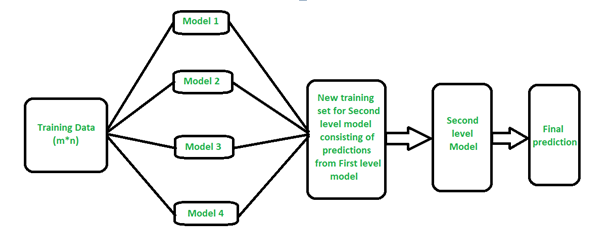
\includegraphics[width=0.45\textwidth]{Ensemble/ensemble.PNG}
	\caption{Ensemble Stacking Model Architecture}
	\label{fig:ensemble}
\end{figure}


Fig \ref{fig:gb_lr} shows the second ensemble model we have used Gradient Boosting and Logistic Regression for our level zero classifier models.

On level zero, model 1, GB, was fitted to the training data-set. This classifier model was used to get a prediction on the test set. Similarly, model 2, Logistic Regression, was fitted to the training data-set and then got the prediction on the test set. After that, both models' predictions were concatenated  for both training and testing data-sets. Now on level one, SVM was used as the third and meta classifier model to use the prediction sets of Gradient Boosting and Logistic Regression as features and get the final prediction.

\begin{figure}[h]
	\centering
	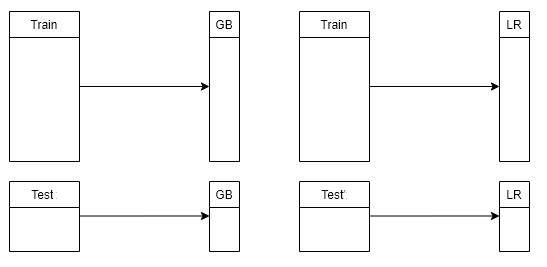
\includegraphics[width=0.45\textwidth]{Ensemble/model2.PNG}
	\caption{GB and LR model prediction set}
	\label{fig:gb_lr}
\end{figure}


For Gradient Boosting, the parameters we have used are,

n\_estimators=100;
It is the number of boosting steps that must be completed. Gradient boosting is somewhat resistant to over-fitting, therefore a big number typically yields better results.

max\_depth=1;
The individual regression estimators' maximum depth. The maximum depth of the tree restricts the number of nodes. Tune this parameter for optimal performance; the optimal value is determined by the interplay of the input variables.

For Logistic Regression,the parameters we have used are,
'penalty': 'l1 ; Used to specify the norm used in the penalization.


'solver' : 'saga'; solver parameter is used as Algorithm to use in the optimization problem. Saga handles l1 penalty.


'tol' :0.1 ; Tolerance for stopping criteria.

	 
\subsubsection{LGBM with Oversampling} \label{subsubsec:lgb_smote}
	 
Imbalanced classification entails creating prediction models for data-sets with a significant class imbalance. When working with unbalanced data-sets, the issue is that most machine learning approaches will disregard the minority class, resulting in poor performance, even though performance on the minority class is generally the most significant. This is exactly what happened with our models.

The data-set used is hugely biased to one class, and the ratio of the class distribution is about 90:10 percent. Although we obtained high accuracy, our accuracy for one class is way below that of another. Oversampling the minority class is one way to deal with unbalanced data-sets. Duplicating instances in the minority class is the easiest technique, but these examples don't provide new information to the model. Instead, new instances may be created by synthesizing old ones. The Synthetic Minority Oversampling Technique, or SMOTE for short, is a kind of data augmentation for the minority population.


Fig \ref{fig:Oversample}  shows that after executing SMOTE on our data-set, the minority class data has been increased, and the data distribution for both the class became equal 50:50 percent. Now we can build our model for an unbiased model.	 

\begin{figure}[t]
	\centering
	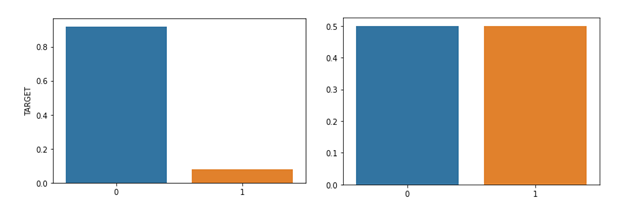
\includegraphics[width=0.45\textwidth]{Oversampling/smote.PNG}
	\caption{data-set Before and after Oversampling using SMOTE}
	\label{fig:Oversample}
\end{figure}


\section{Experiments}
\subsection{Data Description}
The data-set provides a lot of information about the borrower. It is segregated into multiple relational tables, which contain applicants’ static data such as their gender, age, number of family members, occupation, and other related fields, applicant’s previous credit history obtained from the credit bureau department, and the applicant’s past credit history within the Home Credit Group itself. 
For the training file, we have a total of 307511 observations and 122 features to consider with integer, float and object datatype. Also there are 67 features with null value. The test file is almost similar as the training file having 48744 observations, 121 features (minus the predictor variable ’TARGET’), and 64 features having null values. The words being used as; Observations = rows, features= columns based on what we have observed. Only around 8 training set did not repay the loan. The training data is unbalanced, and a significantly higher proportion of people listed in our sample can repay loans, compared to people who default on loans. For each of the 122 features, the correlation coefficient was calculated with the target value.

% Start

\begin{figure*}[t] 
	\centering
	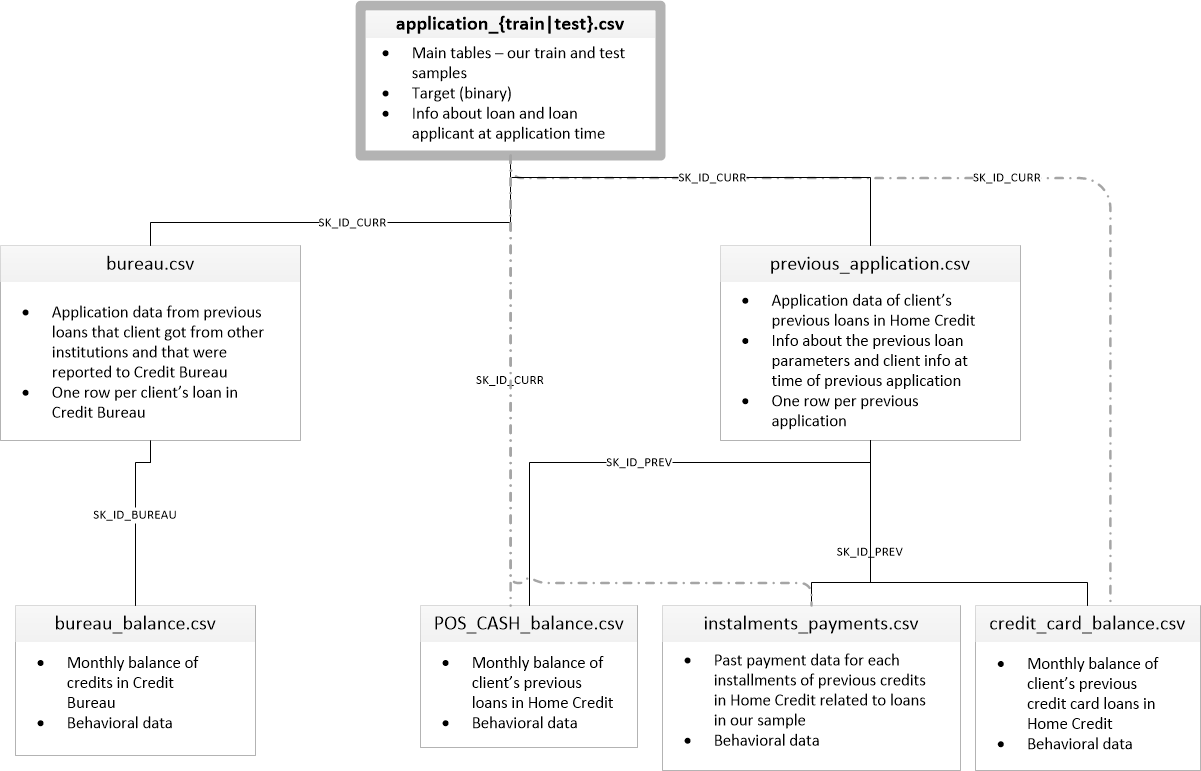
\includegraphics[width=\textwidth]{data/home_credit.png}
	\caption{Data Diagram\cite{Start_Here_:_A_Gentle_Introduction}}
	\label{fig:data_diag}
\end{figure*}

The current application has features such as:
\begin{itemize}
	\item If the applicant has a car or real estate.
	\item Number of descendants of the applicant.
	\item Income of the client and their profession.
	\item Amount of the loan and it's type and purpose.
	\item Level of education.
	\item Family status and living situation.
	\item Number of days they were employed in their current job. 
	\item If the customer has a phone, how long has it been in use.
	\item Details about when and where the loan application was filed.
	\item Normalized score from external credit scorers.
	\item Number of documents submitted.
\end{itemize}

The Home Credit International data on credit bureau includes features such as:
\begin{itemize}
	\item If the applicant has a credit report with basic information such as if it is active and when it was last updated.
	\item The total amount of debt that the applicant currently owes, as well as the specifics of that obligation.
	\item Payment information for prior debts.
\end{itemize}

The data from Home Credit International on previous applications includes details such as:
\begin{itemize}
	\item The loan amount, kind, and it's purpose.
	\item In the application data, there might be many previous loans for each current loan.
	\item Each previous application has one row and is identified by the feature SK\_ID\_PREV.
\end{itemize}

The following are some of the features of the Home Credit International statistics on bureau balance:
\begin{itemize}
	\item Monthly statistics on the bureau's credit history.
	\item A previous credit might have many rows, one for each month of the credit period.
\end{itemize}

The Home Credit International data on POS\_CAS\_BALANCE data includes characteristics such as:
\begin{itemize} 
	\item Monthly data on previous Home Credit point-of-sale or cash-loan transactions.
	\item Each row represents one month of a previous point of sale or cash loan, although a single prior loan could include many rows.
\end{itemize}

The Home Credit International data on credit card balance includes elements such as:
\begin{itemize}
	\item Clients' prior credit cards with Home Credit are tracked on a monthly basis.
	\item Each row represents a month's credit card balance, and each credit card might contain many rows.
\end{itemize}

The Home Credit International data on installment payments includes characteristics such as:
\begin{itemize}
	\item Every made payment has it's own row, and every missed payment has it's own row.
\end{itemize}

\subsection{Baseline} \label{subsec:baseline}

We used a linear model as our baseline. 

\paragraph{Data Pipeline}
It is very similar to \ref{subsubsec:log_reg}, but we did not use the Data processing Pipeline described in \ref{subsec:feat_eng}, instead we just used the application data. We used One-Hot Encoding\cite{sklearn.preprocessing.onehotencoder} to encode the categorical data, remove all positive and negative infinities, use Simple Imputer\cite{sklearn.impute.simpleimputer} and MinMax Scaler\cite{sklearn.preprocessing.minmaxscaler} models to pre-process the data.

\paragraph{Training}
The parameter used for the Logistic Regression model is C=0.0001. 

\paragraph{Score}
The model had an AUC-ROC private score of 0.68453 and a public score of 0.68157. 

\subsection{Evaluation Metrics} \label{subsec:aucroc}

Our evaluation metrics across all models is \emph{Area Under the curve of Receiver Operating Characteristic} curve (AUC-ROC)\cite{narkhede2018understanding}. We chose AUC-ROC score since it shows how good the model is at predicting True Positives. However, we did not have the true values of our test data-set, so we are relied on Kaggle for accuracy score. Kaggle uses AUC-ROC to score our predictions.

Before we understand AUC-ROC, we need to look into Receiver Operating Characteristic (ROC) curve. It is a probability curve of True Positive Rate (TPR) vs False Positive Rate (FPR). The TPR and FPR are on the y and x axis respectively. An example would be Figure \ref{fig:lgb_roc}.

We need a better understanding of TPR and FPR, in order to understand Confusion Matrix. A Confusion Matrix is a matrix of Predicted and Actual target, which is represented in Table \ref{tab:conf_mat}. 

\begin{table}[h]
	\caption{Confusion Matrix}
	\label{tab:conf_mat}
	\begin{tabular}{ll|l|l|}
		\cline{3-4}
		&          & \multicolumn{2}{c|}{True Class} \\ \cline{3-4} 
		                                                       &          & Positive & Negative \\ \hline
		\multicolumn{1}{|c|}{\multirow{2}{*}{Predicted Class}} & Positive & TP       & FP       \\ \cline{2-4} 
		\multicolumn{1}{|c|}{}                                 & Negative & FN       & TN       \\ \hline
	\end{tabular}
\end{table}

True Positive Rate, a.k.a. TPR, Recall, Sensitivity means how accurately a model can predict a true value correctly. The equation to calculate TPR is shown in equation \ref{eqn:tpr}
\begin{equation}
	\label{eqn:tpr}
	TPR = \frac{TP}{TP + FN}
\end{equation}
where:
\begin{conditions}
	TPR     &   True Positive Rate  \\
	TP      &   True Positive       \\
	FN      &   False Negative      \\
\end{conditions}

False Positive Rate is the rate of wrong predictions by a model. The equation to calculate FPR is shown in equation \ref{eqn:fpr}
\begin{equation}
	\label{eqn:spec}
	Specificity = \frac{TN}{TN + FP}
\end{equation}

\begin{equation}
	\label{eqn:fpr}
	FPR = 1 - Specificity
	= \frac{FP}{TN + FP}
\end{equation}
where:
\begin{conditions}
	FPR     &   False Positive Rate  \\
	FP      &   False Positive       \\
	TN      &   True Negative        \\
\end{conditions}

So, a perfect model would have an AUC score of 1 and if a model predicts all classes as 1 then it's AUC will be 0.5. It means the model has no class separation capacity. So a good model would have a higher AUC score between 0.5 and 1.

\section{Results and Discussion}

We have had mixed results from our models. Among all models, Gradient Boosting based models performed much better than other types of models.

Point to be noted, all the scores discussed in this section were obtained from Kaggle. Kaggle computes the AUC-ROC score from the predicted probability of the test data-set we created using our models. And as we do not have the labels for test data-set, we were not able to create Confusion Matrices.

\subsection{Gradient Boosting}

LightGBM (\ref{subsubsec:lgb}) and XGBoost (\ref{subsubsec:xgb}) are the variants of gradient boosting models trained on this data-set. The scores with their corresponding parameters are given in Table \ref{tab:lgb} and \ref{tab:xgb} respectively.

\begin{table*}[t]
	\centering
	\caption{LightGBM Scores}
	\label{tab:lgb}
	\begin{tabular}{@{}|l|l|l|l|l|l|l|@{}}
		\toprule
		\textbf{Run}                     & \textbf{1} & \textbf{2} & \textbf{3} & \textbf{4} & \textbf{5} & \textbf{6} \\ \midrule
		\textbf{Pre-processing Pipeline} & v1         & v1.1       & v1.1       & v1.1       & v1.1       & v1.1       \\ \midrule
		\textbf{boosting\_type}          &            &            &            & goss       & goss       &            \\ \midrule
		\textbf{n\_estimators}           & 10000      & 10000      & 5000       & 5000       & 8888       & 10000      \\ \midrule
		\textbf{early\_stopping\_rounds} & 100        & 100        & 100        & 100        & 2500       & 2500       \\ \midrule
		\textbf{objective}               & binary     & binary     &            &            &            &            \\ \midrule
		\textbf{class\_weight}           & balanced   & balanced   &            &            &            &            \\ \midrule
		\textbf{learning\_rate}          & 0.05       & 0.05       & 0.01       & 0.01       & 0.01       & 0.01       \\ \midrule
		\textbf{reg\_alpha}              & 0.1        & 0.1        & 3.564      & 3.564      & 3.564      & 3.564      \\ \midrule
		\textbf{reg\_lamda}              & 0.1        & 0.1        & 4.9306     & 4.93       & 4.93       & 4.93       \\ \midrule
		\textbf{subsample}               & 0.8        & 0.8        & 0.708      & 0.708      & 0.708      & 0.708      \\ \midrule
		\textbf{n\_jobs}                 & 1          & 1          &            &            &            &            \\ \midrule
		\textbf{random-state}            & 50         & 50         &            & 88888      & 88888      & 88888      \\ \midrule
		\textbf{nthread}                 &            &            & -1         & -1         & -1         & -1         \\ \midrule
		\textbf{max\_depth}              &            &            & 11         & 11         & 11         & 11         \\ \midrule
		\textbf{num\_leaves}             &            &            & 58         & 58         & 58         & 58         \\ \midrule
		\textbf{colsample\_bytree}       &            &            & 0.613      & 0.613      & 0.613      & 0.613      \\ \midrule
		\textbf{max\_bin}                &            &            & 407        & 407        & 407        & 407        \\ \midrule
		\textbf{min\_child\_weight}      &            &            & 6          & 6          & 6          & 6          \\ \midrule
		\textbf{min\_child\_samples}     &            &            & 165        & 165        & 165        & 165        \\ \midrule
		\textbf{silent}                  &            &            & -1         & -1         & -1         & -1         \\ \midrule
		\textbf{verbose}                 &            &            & -1         & -1         & -1         & -1         \\ \midrule
		\textbf{private\_score}          & 0.78489    & 0.79235    & 0.7973     & 0.79817    & 0.79750    & 0.79702    \\ \midrule
		\textbf{public\_score}           & 0.7871     & 0.794      & 0.80123    & 0.79998    & 0.80035    & 0.80101    \\ \bottomrule
	\end{tabular}
\end{table*}

\begin{table*}[t]
	\centering
	\caption{XGBoost Scores}
	\label{tab:xgb}
	\begin{tabular}{@{}|l|l|l|l|l|l|@{}}
		\toprule
		\textbf{Run}                     & \textbf{1} & \textbf{2} & \textbf{3}     & \textbf{4}     \\ \midrule
		\textbf{Pre-processing Pipeline} & v1         & v1.1       & v1.1           & v1.1           \\ \midrule
		\textbf{kfolds}                  &            &            & 5              & 5              \\ \midrule
		\textbf{kfolds\_random}          &            &            &                & 8888           \\ \midrule
		\textbf{tree\_method}            &            &            & gpu\_hist      & gpu\_hist      \\ \midrule
		\textbf{predictor}               &            &            & gpu\_predictor & gpu\_predictor \\ \midrule
		\textbf{n\_estimators}           & 1200       & 1200       & 5000           & 5000           \\ \midrule
		\textbf{early\_stopping\-rounds} & 100        & 100        & 2500           & 2500           \\ \midrule
		\textbf{learning\_rate}          &            &            & 0.01           & 0.01           \\ \midrule
		\textbf{max\_depth}              &            &            & 11             & 11             \\ \midrule
		\textbf{gamma}                   & 0.098      & 0.098      & 0.098          & 0.098          \\ \midrule
		\textbf{subsample}               & 0.5        & 0.5        & 0.708          & 0.708          \\ \midrule
		\textbf{reg\_alpha}              &            &            & 3.564          & 3.564          \\ \midrule
		\textbf{reg\_lambda}             &            &            & 4.93           & 4.93           \\ \midrule
		\textbf{random\_state}           &            &            &                & 8888           \\ \midrule
		\textbf{seed}                    &            &            &                & 88888          \\ \midrule
		\textbf{colsample\_bytree}       &            &            & 0.613          & 0.613          \\ \midrule
		\textbf{min\_child\_weight}      &            &            & 6              & 6              \\ \midrule
		\textbf{private\_score}          & 0.75581    & 0.76317    & 0.79232        & 0.78410        \\ \midrule
		\textbf{public\_score}           & 0.75958    & 0.76661    & 0.7962         & 0.78710        \\ \bottomrule
	\end{tabular}
\end{table*}

We also trained a LightGBM model with oversampling using SMOTE. The scores are given in Table \ref{tab:lgb_smote}.

\begin{table}[h]
	\caption{Score of LightGBM using SMOTE}
	\label{tab:lgb_smote}
	\begin{tabular}{@{}|l|l|l|@{}}
		\toprule
		\textbf{Model}            & \textbf{Public Score} & \textbf{Private Score} \\ \midrule
		\textbf{LGBM using SMOTE} & 0.75513               & 0.75949                \\ \bottomrule
	\end{tabular}
\end{table} 

LightGBM performed better between the two models. Our speculation is that, LightGBM performed better because of it's unique feature where it only grows leaves with the highest delta in cost function, whereas XGBoost grows the level of the tree. This is why LightGBM models train faster on data-sets with many features than XGBoost with lower memory consumption.

Although we can see that the models performed much better than our Baseline model (\ref{subsec:baseline}) becasuse of using better Data Pipeline and better ML models. The models particularly improved performance with Data Pieline v1.1 (\ref{data:v1.1}) because Gradient Boosting Trees perform better with more features.

The ROC curve of the best performing LightGBM model with the training data-set is given in Figure \ref{fig:lgb_roc}

\begin{figure}[h]
	\centering
	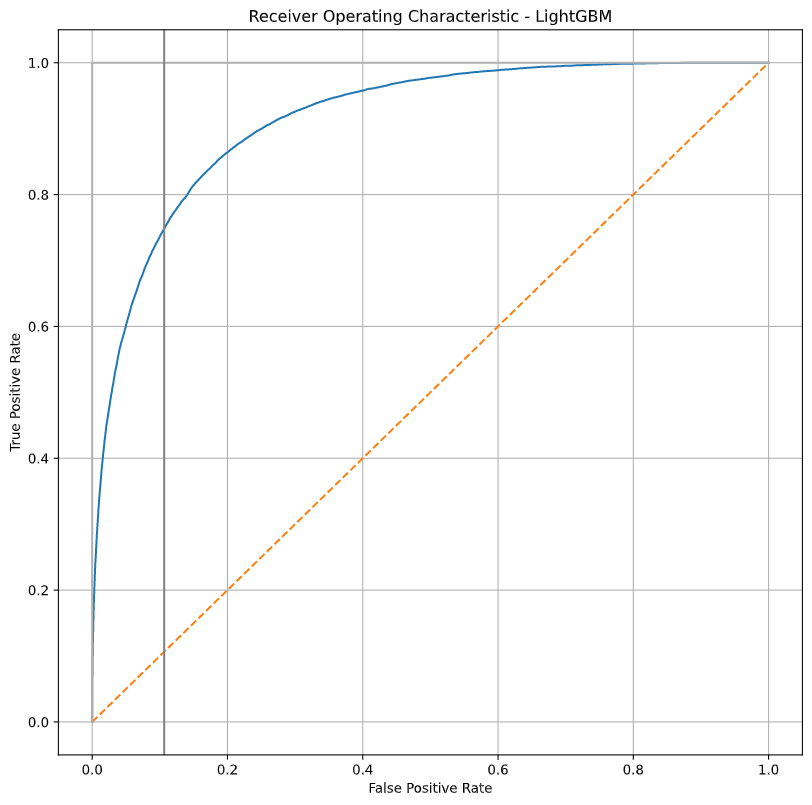
\includegraphics[width=0.45\textwidth]{lgb/roc}
	\caption{ROC Curve of LightGBM}
	\label{fig:lgb_roc}
\end{figure}

The ROC Curve with the best scoring model can be seen in Figure \ref{fig:xgb_roc}
\begin{figure}[h]
	\centering
	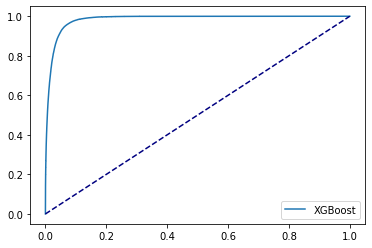
\includegraphics[width=0.45\textwidth]{xgb/roc.png}
	\caption{ROC Curve of XGBoost}
	\label{fig:xgb_roc}
\end{figure}

\subsection{Deep Learning}

\begin{table}[h]
	\caption{TabNet Scores}
	\label{tab:tabnet}
	\begin{tabular}{@{}|l|l|l|l|@{}}
		\toprule
		\textbf{Run}                  & \textbf{1} & \textbf{2} & \textbf{3} \\ \midrule
		\textbf{Data Pipeline}        & v1         & v1.1       & v1.1       \\ \midrule
		\textbf{kfolds}               &            &            & 5          \\ \midrule
		\textbf{step\_size}           & 10         & 10         & 20         \\ \midrule
		\textbf{gamma}                & 0.9        & 0.9        & 0.95       \\ \midrule
		\textbf{mask\_type}           & entmax     & entmax     &            \\ \midrule
		\textbf{patience}             & 50         & 50         & 50         \\ \midrule
		\textbf{batch\_size}          & 256        & 256        & 1024       \\ \midrule
		\textbf{virtual\_batch\_size} & 128        & 128        & 128        \\ \midrule
		\textbf{num\_workers}         & 0          & 0          & 0          \\ \midrule
		\textbf{weights}              & 1          & 1          & 1          \\ \midrule
		\textbf{drop\_last}           & False      & False      & False      \\ \midrule
		\textbf{n\_d}                 &            &            & 32         \\ \midrule
		\textbf{n\_a}                 &            &            & 32         \\ \midrule
		\textbf{n\_step}              &            &            & 10         \\ \midrule
		\textbf{gamma}                &            &            & 0.098      \\ \midrule
		\textbf{n\_independnet}       &            &            & 2          \\ \midrule
		\textbf{n\_shared}            &            &            & 2          \\ \midrule
		\textbf{lamda\_sparse}        &            &            & $1e^{-3}$  \\ \midrule
		\textbf{momentum}             &            &            & 0.4        \\ \midrule
		\textbf{clip\_value}          &            &            & 2          \\ \midrule
		\textbf{epsilon}              &            &            & $1e^{-15}$ \\ \midrule
		\textbf{private\_score}       & 0.75436    & 0.71452    & 0.76985    \\ \midrule
		\textbf{public\_score}        & 0.76380    & 0.71391    & 0.77980    \\  \bottomrule
	\end{tabular}
\end{table}

A deep learning TabNet (\ref{subsubsec:tabnet}) model was trained using our Processed Data (\ref{subsec:feat_eng}). The scores of TabNet are given in table \ref{tab:tabnet}.

We can see that the Deep Learning TabNet model performs better with lower number of features when trained with a CPU. Possibly because the model doesn't have a technique to ignore features with lower weights. When the model is trained using a CPU, a possible improvement would be to look at the feature and their weights and drop the features with lowest weights (an arbitrary threshold can be set) to train the model. That should yield better score than our current ones. Although that limitation can be overcome by training the model with a CUDA enable GPU with enough VRAM. The model accesses the VRAM of the GPU to store the tensors as well as the system memory. Thus training with a system with faster RAM (3200 MHz+ DDR4) and higher bandwidth memory (GDDR5X+) yields better scores. 

Since Deep Learning models for tabular data are still in their early stages, further development of similar techniques have the potential to perform better or atleast similar to Gradient Boosting Machines.

\subsection{Neural Networks}

\begin{table}[h]
	\caption{Neural Network Embedding Scores}
	\label{tab:emb}
	\begin{tabular}{@{}|l|l|l|l|@{}}
		\toprule
		\textbf{Run}               & \textbf{1} & \textbf{2} & \textbf{3}           \\ \midrule
		\textbf{kfolds}            & 5          & 7          & 6                    \\ \midrule
		\textbf{Shuffle}           & True       & True       & True                 \\ \midrule
		\textbf{Random State}      & 1          & 1          & 1                    \\ \midrule
		\textbf{optimizer}         & Adam       & Adam       & Adam                 \\ \midrule
		\textbf{patience}          & 10         & 5          & 5                    \\ \midrule
		\textbf{scaler}            &            &            & minmaxscaler         \\ \midrule
		\textbf{max\_epoch}        & 250        & 150        & 250                  \\ \midrule
		\textbf{loss}              &            &            & binary\_crossentropy \\ \midrule
		\textbf{private\_score}    & 0.7500     & 0.7513     & 0.7500               \\ \midrule
		\textbf{public\_score}     & 0.7455     & 0.7492     & 0.7489               \\  \bottomrule
	\end{tabular}
\end{table}

\begin{figure}[h]
	\centering
	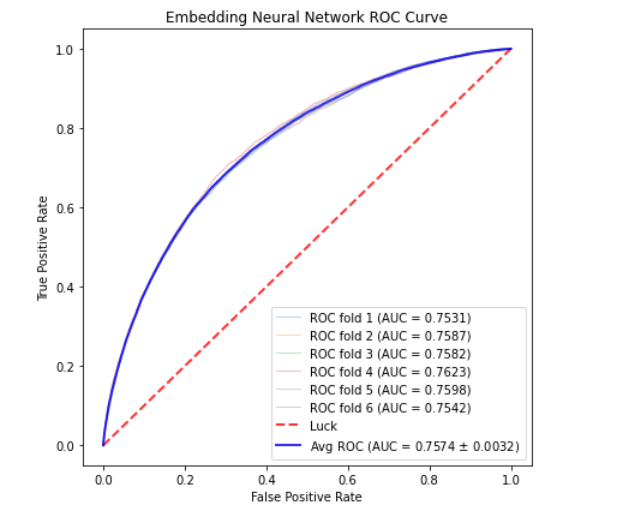
\includegraphics[width=0.45\textwidth]{embedding_nn/ROC-AUC.PNG}
	\caption{Embedding NN ROC Curve}
	\label{fig:embedding_nn_roc}
\end{figure}

\begin{figure}[h]
	\centering
	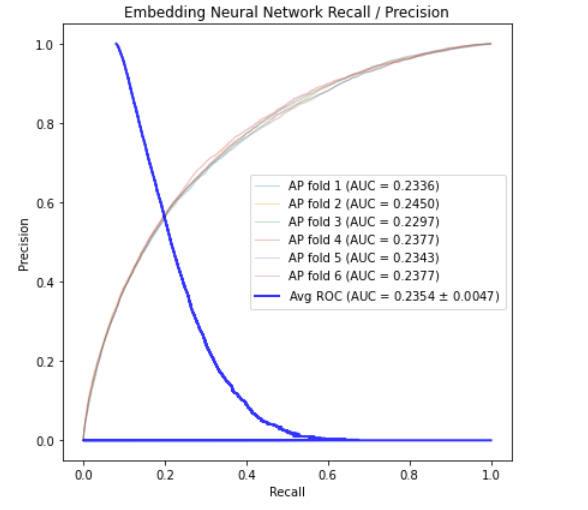
\includegraphics[width=0.45\textwidth]{embedding_nn/Precision.PNG}
	\caption{Embedding NN Recall/Precision Curve}
	\label{fig:embedding_nn_recall}
\end{figure}

\begin{table}[h]
	\caption{Neural Network Scores}
	\label{tab:nn_pial}
	\begin{tabular}{@{}|l|l|l|@{}}
		\toprule
		\textbf{Run}            & \textbf{1} & \textbf{2} \\ \midrule
		\textbf{Iterations}     & 41         & 10         \\ \midrule
		\textbf{private\_score} & 0.73427    & 0.75763    \\ \midrule
		\textbf{public\_score}  & 0.72862    & 0.75533    \\ \bottomrule
	\end{tabular}
\end{table}  

We trained a few neural network models with major differences between their network configuration. But none of the models we trained have shown promising scores. Mostly because of the infinite possibility of network configuration and other parameter tests, we could not find a model that performed close to our Gradient Boosting Trees. We believe further training of Neural Networks with different network configuration and fine-tuning of their paramaters should help the models classify the data-set better. The scores of our Neural Network models are given in Table \ref{tab:emb} \& \ref{tab:nn_pial}.

\subsection{Ensemble Model}

The ensemble model described in \ref{subsubsec:ensemble} procudes the scores in table \ref{tab:ensemble}.
\begin{table}[h]
	\caption{Private and Public score of ensemble model}
	\label{tab:ensemble}
	\begin{tabular}{@{}|l|l|l|@{}}
		\toprule
		\textbf{Model}          & \textbf{Public Score} & \textbf{Private Score} \\ \midrule
		\textbf{Stacking Model} & 0.71996               & 0.72819                \\ \midrule
	\end{tabular}
\end{table}

\begin{table}[h]
	\caption{Weighted Avg between XGBoost and LightGBM}
	\label{tab:wa_2}
	\begin{tabular}{@{}|l|l|l|@{}}
		\toprule
		\textbf{Model}            & \textbf{Public Score} & \textbf{Private Score} \\ \midrule
		\textbf{XGBoost}          & 0.76661               & 0.76317                \\ \midrule
		\textbf{LightGBM}         & 0.79411               & 0.79092                \\ \midrule
		\textbf{Weighted Average} & 0.78851               & 0.78838                \\ \bottomrule
	\end{tabular}
\end{table} 

\begin{table}[h]
	\caption{Weighted Avg: Embedding NN and LightGBM}
	\label{tab:wa_1}
	\begin{tabular}{@{}|l|l|l|@{}}
		\toprule
		\textbf{Model}            & \textbf{Public Score} & \textbf{Private Score} \\ \midrule
		\textbf{Embedding NN}     & 0.74603               & 0.75052                \\ \midrule
		\textbf{LightGBM}         & 0.79411               & 0.79092                \\ \midrule
		\textbf{Weighted Average} & 0.78852               & 0.78802                \\ \bottomrule
	\end{tabular}
\end{table} 

We created some simple ensemble models using the weighted average technique in \ref{subsubsec:wa_1} and \ref{tab:wa_2}. We believe if we use Grid Search technique\cite{sklearn.model_selection.gridsearchcv} to determine the weights and use scores from the top 3 different types of best performing models, we would have better scores.

\subsection{Logistic Regression}

This is the simplest model we experimented with. The model performs very well, compared to other simpler models. This is the closest relative to our baseline model and it yield better scores simply due to the association of the Feature Engineered Pipeline. The scores of Logistic Regression model is given in Table \ref{tab:log_reg}.

\begin{table}[h]
	\caption{Logistic Regression Scores}
	\label{tab:log_reg}
	\begin{tabular}{@{}|l|l|l|@{}}
		\toprule
		\textbf{Run}             & \textbf{1} & \textbf{2} \\ \midrule
		\textbf{Data Processing} & v1         & v1.1       \\ \midrule
		\textbf{C}               & 0.0001     & 0.0001     \\ \midrule
		\textbf{private\_score}  & 0.72880    & 0.73428    \\ \midrule
		\textbf{public\_score}   & 0.73723    & 0.73962    \\ \bottomrule
	\end{tabular}
\end{table}

\subsection{Random Forest}

Random Forest worked very well compared to how simple it's implementation is and how minimum memory and time it requires to train. A bigger ensemble (higher number of estimators) of Random Forest and a Neural Networks should have yield better scores. The scores of Random Forest model is given in Table \ref{tab:ran_for}.

\begin{table}[h]
    \caption{Random Forest}
    \label{tab:ran_for}
    \begin{tabular}{@{}|l|l|l|@{}}
        \toprule
        \textbf{Run}            & \textbf{1} & \textbf{2} \\ \midrule
        \textbf{Data Pipeline}  & v1         & v1.1       \\ \midrule
        \textbf{n\_estimators}  & 100        & 100        \\ \midrule
        \textbf{random\_state}  & 50         & 50         \\ \midrule
        \textbf{verbose}        & 1          & 1          \\ \midrule
        \textbf{n\_jobs}        & -1         & -1         \\ \midrule
        \textbf{private\_score} & 0.72070    & 0.72396    \\ \midrule
        \textbf{public\_score}  & 0.71386    & 0.73139    \\ \bottomrule
    \end{tabular}
\end{table}

\subsection{Comparison between all models and Baseline}

We have tested a lot of different classifier models and we believe a direct comparison with the Baseline would contrast our findings much better in Table \ref{tab:all}.

\begin{table*}[t]
    \caption{Score Comparison of all models}
    \label{tab:all}
    \begin{tabular}{@{}|c|l|l|l|@{}}
        \toprule
\multicolumn{1}{|l|}{\textbf{Data   PipeLine}} & \textbf{Model}                                                & \textbf{private\_score} & \textbf{public\_score} \\ \midrule
\multicolumn{1}{|l|}{\textbf{}} & \textbf{Baseline}            & 0.68453 & 0.68157 \\ \midrule
\multirow{5}{*}{\textbf{v1}}    & \textbf{Logistic Regression} & 0.7288  & 0.73723 \\ \cmidrule(l){2-4} 
                                & \textbf{Random Forest}       & 0.7207  & 0.71386 \\ \cmidrule(l){2-4} 
                                & \textbf{LightGBM}            & 0.78489 & 0.7871  \\ \cmidrule(l){2-4} 
                                & \textbf{XGBoost}             & 0.75581 & 0.75958 \\ \cmidrule(l){2-4} 
                                & \textbf{TabNet}              & 0.75436 & 0.7638  \\ \midrule
\multirow{5}{*}{\textbf{v1.1}}  & \textbf{Logistic Regression} & 0.73428 & 0.73962 \\ \cmidrule(l){2-4} 
                                & \textbf{Random Forest}       & 0.72396 & 0.73139 \\ \cmidrule(l){2-4} 
                                & \textbf{LightGBM}            & 0.7973  & 0.80123 \\ \cmidrule(l){2-4} 
                                & \textbf{XGBoost}             & 0.79232 & 0.7962  \\ \cmidrule(l){2-4} 
                                & \textbf{TabNet}              & 0.76985 & 0.7798  \\ \midrule
\multicolumn{1}{|l|}{\textbf{}} & \textbf{LightGBM SMOTE}      & 0.75949 & 0.75513 \\ \midrule
\multicolumn{1}{|l|}{\textbf{}}                & \textbf{Neural Network   Embedding}                           & 0.7513                  & 0.7492                 \\ \midrule
\multicolumn{1}{|l|}{\textbf{}} & \textbf{Neural Network}      & 0.75763 & 0.75533 \\ \midrule
\multicolumn{1}{|l|}{\textbf{}} & \textbf{Ensemble}            & 0.72819 & 0.71996 \\ \midrule
\multicolumn{1}{|l|}{\textbf{}}                & \textbf{Weighted Average 1}                  & 0.78802                 & 0.78852                \\ \midrule
\multicolumn{1}{|l|}{\textbf{}}                & \textbf{Weighted Average 2} & 0.78838                 & 0.78851                \\ \bottomrule
\end{tabular}
\end{table*}

We can see a trend of Gradient Boosting based classifier performing much better than other types. Although if the suggested improvements were made to Neural Networks and an upgraded Deep Learning Model was used, it should be able to perform the same, if not better than the Gradient Boosting models. And a much computed heavy solution would be, to use weighted average if the suggested improvements were made.

% End

\section{Conclusion}

Most of the training was performed with widely accepted binary classifier models. Since, the data-set is unbalanced to a ratio of 10:1, our
models were better at predicting True Positives than False Negatives. Translating that to real work scenario, our models were able to predict the applicants who was more likely to pay back the loan versus those who aren't.

Our best AUC-ROC score was 0.80123, which means it accurately predicted 80.123\% of both classes combined. In a production environment this accuracy is not enough unless there are other mechanisms deployed to assist it. A credit assessment score similar to what Equifax, TransUnion provides using a Regression Algorithm would be a better risk assessment tool than a Classifier Algorithm used in our work.

In our testing, we have figured that Deep Learning for Tabular Data is not advanced enough to compete with Gradient Boosting Algorithms.even though the development of such models look very promising. Moreover, Neural Network based models have the potential to perform similar, if not better than Gradient Boosting Models.

A regression algorithm would provide an overall score to the credit-ability and the financial overview of the applicant. Lenders can use this information to achieve better data driven decision.

A classifier algorithm, demonstrated in our work, is an excellent tool to pre-approve or shortlist loan applications. But using such algorithm as a decision making tool would not be wise at this stage. Although further research on such algorithm should yield better results.

\bibliographystyle{ACM-Reference-Format}
\bibliography{ref}


\section*{APPENDIX A}
\subsection*{Regarding the accuracy and hardware performance relationship in TabNet}

We established a relationship between a TabNet Classifier model's accuracy with the hardware performance. We ran the model multiple times in a three different hardware with the same code-base but found slightly different results. We figured that the the model performing slightly better on GPUs with larger and faster VRAM and faster access to system Memory.

The systems we tested the model and ranking in accuracy are:
\begin{description}

    \item[Kaggle Notebook] GPU: NVIDIA Tesla P100, RAM: 15 GB DDR4
    \item[Google Colab Notebook] GPU: NVIDIA Tesla K80, RAM: 13 GB DDR4
    \item[Custom PC] GPU: NVIDIA GTX 1080, RAM: 32 GB DDR4
    
\end{description}

\subsection*{LightGBM Boosting Type's effect on Memory Optimization}

We also figured that when LightGBM's boosting type is used in parameters, which are Gradient-Based One-Side Sampling (GOSS) and Exclusive Feature Bundling (EFB), the model uses almost half the memory to train while still retaining the original accuracy. This is because the boosting methods drop features with smaller importance.

\end{document}
\endinput